\documentclass[11pt,compress,t,notes=noshow, xcolor=table]{beamer}
\usepackage[]{graphicx}\usepackage[]{color}
% maxwidth is the original width if it is less than linewidth
% otherwise use linewidth (to make sure the graphics do not exceed the margin)
\makeatletter
\def\maxwidth{ %
  \ifdim\Gin@nat@width>\linewidth
    \linewidth
  \else
    \Gin@nat@width
  \fi
}
\makeatother

\definecolor{fgcolor}{rgb}{0.345, 0.345, 0.345}
\newcommand{\hlnum}[1]{\textcolor[rgb]{0.686,0.059,0.569}{#1}}%
\newcommand{\hlstr}[1]{\textcolor[rgb]{0.192,0.494,0.8}{#1}}%
\newcommand{\hlcom}[1]{\textcolor[rgb]{0.678,0.584,0.686}{\textit{#1}}}%
\newcommand{\hlopt}[1]{\textcolor[rgb]{0,0,0}{#1}}%
\newcommand{\hlstd}[1]{\textcolor[rgb]{0.345,0.345,0.345}{#1}}%
\newcommand{\hlkwa}[1]{\textcolor[rgb]{0.161,0.373,0.58}{\textbf{#1}}}%
\newcommand{\hlkwb}[1]{\textcolor[rgb]{0.69,0.353,0.396}{#1}}%
\newcommand{\hlkwc}[1]{\textcolor[rgb]{0.333,0.667,0.333}{#1}}%
\newcommand{\hlkwd}[1]{\textcolor[rgb]{0.737,0.353,0.396}{\textbf{#1}}}%
\let\hlipl\hlkwb

\usepackage{framed}
\makeatletter
\newenvironment{kframe}{%
 \def\at@end@of@kframe{}%
 \ifinner\ifhmode%
  \def\at@end@of@kframe{\end{minipage}}%
  \begin{minipage}{\columnwidth}%
 \fi\fi%
 \def\FrameCommand##1{\hskip\@totalleftmargin \hskip-\fboxsep
 \colorbox{shadecolor}{##1}\hskip-\fboxsep
     % There is no \\@totalrightmargin, so:
     \hskip-\linewidth \hskip-\@totalleftmargin \hskip\columnwidth}%
 \MakeFramed {\advance\hsize-\width
   \@totalleftmargin\z@ \linewidth\hsize
   \@setminipage}}%
 {\par\unskip\endMakeFramed%
 \at@end@of@kframe}
\makeatother

\definecolor{shadecolor}{rgb}{.97, .97, .97}
\definecolor{messagecolor}{rgb}{0, 0, 0}
\definecolor{warningcolor}{rgb}{1, 0, 1}
\definecolor{errorcolor}{rgb}{1, 0, 0}
\newenvironment{knitrout}{}{} % an empty environment to be redefined in TeX

\usepackage{alltt}
\newcommand{\SweaveOpts}[1]{}  % do not interfere with LaTeX
\newcommand{\SweaveInput}[1]{} % because they are not real TeX commands
\newcommand{\Sexpr}[1]{}       % will only be parsed by R
\newcommand{\xmark}{\ding{55}}%


\usepackage[english]{babel}
\usepackage[utf8]{inputenc}

\usepackage{dsfont}
\usepackage{verbatim}
\usepackage{amsmath}
\usepackage{amsfonts}
\usepackage{amssymb}
\usepackage{bm}
\usepackage{csquotes}
\usepackage{multirow}
\usepackage{longtable}
\usepackage{booktabs}
\usepackage{enumerate}
\usepackage[absolute,overlay]{textpos}
\usepackage{psfrag}
\usepackage{algorithm}
\usepackage{algpseudocode}
\usepackage{eqnarray}
\usepackage{arydshln}
\usepackage{tabularx}
\usepackage{placeins}
\usepackage{tikz}
\usepackage{setspace}
\usepackage{colortbl}
\usepackage{mathtools}
\usepackage{wrapfig}
\usepackage{bm}
\usepackage{amsmath}
\usepackage{pifont}
\usepackage{xcolor} %colored math symbols

\usetikzlibrary{shapes,arrows,automata,positioning,calc,chains,trees, shadows}
\tikzset{
  %Define standard arrow tip
  >=stealth',
  %Define style for boxes
  punkt/.style={
    rectangle,
    rounded corners,
    draw=black, very thick,
    text width=6.5em,
    minimum height=2em,
    text centered},
  % Define arrow style
  pil/.style={
    ->,
    thick,
    shorten <=2pt,
    shorten >=2pt,}
}

\usepackage{subfig}

% Defines macros and environments
\usepackage{../../style/lmu-lecture}


\let\code=\texttt
\let\proglang=\textsf

\setkeys{Gin}{width=0.9\textwidth}

\setbeamertemplate{frametitle}{\expandafter\uppercase\expandafter\insertframetitle}

\usepackage{bbm}
% basic latex stuff
\newcommand{\pkg}[1]{{\fontseries{b}\selectfont #1}} %fontstyle for R packages
\newcommand{\lz}{\vspace{0.5cm}} %vertical space
\newcommand{\dlz}{\vspace{1cm}} %double vertical space
\newcommand{\oneliner}[1] % Oneliner for important statements
{\begin{block}{}\begin{center}\begin{Large}#1\end{Large}\end{center}\end{block}}


%new environments
\newenvironment{vbframe}  %frame with breaks and verbatim
{
 \begin{frame}[containsverbatim,allowframebreaks]
}
{
\end{frame}
}

\newenvironment{vframe}  %frame with verbatim without breaks (to avoid numbering one slided frames)
{
 \begin{frame}[containsverbatim]
}
{
\end{frame}
}

\newenvironment{blocki}[1]   % itemize block
{
 \begin{block}{#1}\begin{itemize}
}
{
\end{itemize}\end{block}
}

\newenvironment{fragileframe}[2]{  %fragile frame with framebreaks
\begin{frame}[allowframebreaks, fragile, environment = fragileframe]
\frametitle{#1}
#2}
{\end{frame}}


\newcommand{\myframe}[2]{  %short for frame with framebreaks
\begin{frame}[allowframebreaks]
\frametitle{#1}
#2
\end{frame}}

\newcommand{\remark}[1]{
  \textbf{Remark:} #1
}


\newenvironment{deleteframe}
{
\begingroup
\usebackgroundtemplate{
\includegraphics[width=\paperwidth,height=\paperheight]{../style/color/red.png}}
 \begin{frame}
}
{
\end{frame}
\endgroup
}
\newenvironment{simplifyframe}
{
\begingroup
\usebackgroundtemplate{
\includegraphics[width=\paperwidth,height=\paperheight]{../style/color/yellow.png}}
 \begin{frame}
}
{
\end{frame}
\endgroup
}\newenvironment{draftframe}
{
\begingroup
\usebackgroundtemplate{
\includegraphics[width=\paperwidth,height=\paperheight]{../style/color/green.jpg}}
 \begin{frame}
}
{
\end{frame}
\endgroup
}
% https://tex.stackexchange.com/a/261480: textcolor that works in mathmode
\makeatletter
\renewcommand*{\@textcolor}[3]{%
  \protect\leavevmode
  \begingroup
    \color#1{#2}#3%
  \endgroup
}
\makeatother


\input{../../latex-math/basic-math}
\input{../../latex-math/basic-ml}
\input{../../latex-math/ml-nn}


\newcommand{\titlefigure}{figure/unnamed-chunk-5-4}
\newcommand{\learninggoals}{
  \item Universal approximation theorem for one-hidden-layer neural networks
  \item The pros and cons of a low approximation error 
}

\title{Deep Learning}
\date{}

\begin{document}


\lecturechapter{Universal Approximation}
\lecture{I2DL}

%\section{Universal Approximation}

\begin{vbframe}{Universal approximation property}

  \textbf{Theorem.}
  Let $\sigma : \R \to \R$ be a continuous, non-constant, bounded, and
  monotonically increasing function. Let $C \subset \R^p$ be compact,
  and let $\continuous(C)$ denote the space of continuous functions $C \to \R$.
  Then, given a function $g \in \continuous(C)$ and an accuracy $\varepsilon > 0$,
  there exists a hidden layer size $m \in \N$ and a set of coefficients
  $W_j \in \R^p$, $u_j, b_j \in \R$
  (for $j \in \{1, \dots, m\}$), such that
  $$
    f : C \to \R \,;\quad f(\mathbf{x}) = \sum_{j=1}^m u_j \cdot \sigma \Big( W_j^T \mathbf{x} + b_j \Big)
  $$
  is an $\varepsilon$-approximation of $g$, that is,
  $$
    \|f - g\|_{\infty} := \max_{x \in C} |f(\mathbf{x}) - g(\mathbf{x})| < \varepsilon
    \enspace.
  $$

  The theorem extends trivially to multiple outputs.

  \framebreak

  \textbf{Corollary.}
  Neural networks with a single sigmoidal hidden layer and linear
  output layer are universal approximators.

  \begin{itemize}
    \item This means that for a given target function $g$ there exists a
    sequence of networks $\big( f_k \big)_{k \in \N}$ that converges
    (pointwise) to $g$.%he target function.
    \vspace{2mm}
    \item Usually, as the networks come closer and closer to $g$, they
    will need more and more hidden neurons.
    \vspace{2mm}
    \item A network with fixed layer sizes can only model a subspace of all
    continuous functions. % Its dimensionality is limited by the number
    %of weights.
    \vspace{2mm}
    \item The continuous functions form an infinite dimensional vector space.
    Therefore arbitrarily large hidden layer sizes are needed.
  \end{itemize}

  \framebreak

  \begin{itemize}
  \item Why is universal approximation a desirable property?
  \vspace{2mm}
  \item Recall the definition of a Bayes optimal hypothesis $f^* : X \to Y$.
    It is the best possible hypothesis (model) for the given problem:
    it has minimal loss averaged over the data generating distribution.
  \vspace{2mm}
  \item So ideally we would like the neural network (or any other
    learner) to approximate the Bayes optimal hypothesis.
  \vspace{2mm}
  \item Usually we do not manage to learn $f^*$.
  \vspace{2mm}
  \item This is because we do not have enough (infinite) data. We have
    no control over this, so we have to live with this limitation.
  \vspace{2mm}
  \item But we do have control over which model class we use.
  \end{itemize}

  \framebreak

  \begin{itemize}
    \vspace{10mm}
    \item Universal approximation $\Rightarrow$ approximation error tends
    to zero as hidden layer size tends to infinity.
    \vspace{5mm}
    \item Positive approximation error implies that no matter  how %good the data, 
    big the data set, we cannot find the optimal model.
    \vspace{5mm}
    \item This bears the risk of systematic under-fitting, which can be avoided with a universal model class.
  \end{itemize}

  \framebreak

  \begin{itemize}
    \vspace{5mm}
    \item As we know, there are also good reasons for restricting the model class.
    \vspace{5mm}
    \item This is because a flexible model class with universal approximation
    ability often results in over-fitting, which is no better than
    under-fitting.
    \vspace{5mm}
    \item Thus, \enquote{universal approximation $\Rightarrow$ low approximation error}, but at the risk of a substantial learning error.
    \vspace{5mm}
    \item In general, models of intermediate flexibility give the best predictions.
    For neural networks this amounts to a reasonably sized hidden layer.
  \end{itemize}
\end{vbframe}
%%%%%%%%%%%%%%%%%%%%%%%%%%%%%%%%%%%%%%%%%%%%%%%%%%%%%%%%%%%%%%%%%%
%%%%%%%%%%%%%%%%%%%%%%%%%%%%%%%%%%%%%%%%%%%%%%%%%%%%%%%%%%%%%%%%%%

%%%%%%%%%%%%%%%%%%%%%%%%%%%%%%%%%%%%%%%%%%%%%%%%%%%%%%%%%%%%%%%%%%
%%%%%%%%%%%%%%%%%%%%%%%%%%%%%%%%%%%%%%%%%%%%%%%%%%%%%%%%%%%%%%%%%%
\begin{frame} {Example : Regression/Classification}
  \begin{itemize}
    \vspace{15mm}
    \item Let's look at a few examples of the types of functions and decisions boundaries learnt by neural networks (with a \textbf{single} hidden layer) of various sizes.
        \vspace{5mm}
        \item "size" here refers to the number of neurons in the hidden layer.
    \vspace{5mm}
    %\item The number of "iterations" in the following slides is the number of steps of (stochastic) gradient descent performed.
    \item The number of "iterations" in the following slides corresponds to the number of steps of the applied iterative optimization algorithm (stochastic gradient descent).
  \end{itemize}
\end{frame}

% \begin{vbframe}{Regression: 100 training iterations}
% <<echo=FALSE, warning=FALSE, message=FALSE, results="hide">>=
% 
% library("mlr")
% set.seed(1234L)
% n = 50L
% x = sort(10 * runif(n))
% y = sin(x) + 0.2 * rnorm(x)
% df = data.frame(x = x, y = y)
% tsk = makeRegrTask("sine function example", data = df, target = "y")
% plotLearnerPrediction("regr.nnet", tsk, size = 1L, maxit = 100)
% 
% plotLearnerPrediction("regr.nnet", tsk, size = 2L, maxit = 100)
% 
% plotLearnerPrediction("regr.nnet", tsk, size = 3L, maxit = 100)
% 
% plotLearnerPrediction("regr.nnet", tsk, size = 4L, maxit = 100)
% 
% plotLearnerPrediction("regr.nnet", tsk, size = 5L, maxit = 100)
% 
% plotLearnerPrediction("regr.nnet", tsk, size = 6L, maxit = 100)
% 
% plotLearnerPrediction("regr.nnet", tsk, size = 100L, maxit = 100)
% 
% @
% \end{vbframe}
%%%%%%%%%%%%%%%%%%%%%%%%%%%%%%%%%%%%%%%%%%%%%%%%%%%%%%%%%%%%%%%%%%
%%%%%%%%%%%%%%%%%%%%%%%%%%%%%%%%%%%%%%%%%%%%%%%%%%%%%%%%%%%%%%%%%%
\begin{vbframe}{Regression Ex.: 1000 training iterations}
\begin{knitrout}\scriptsize
\definecolor{shadecolor}{rgb}{0.969, 0.969, 0.969}\color{fgcolor}

{\centering 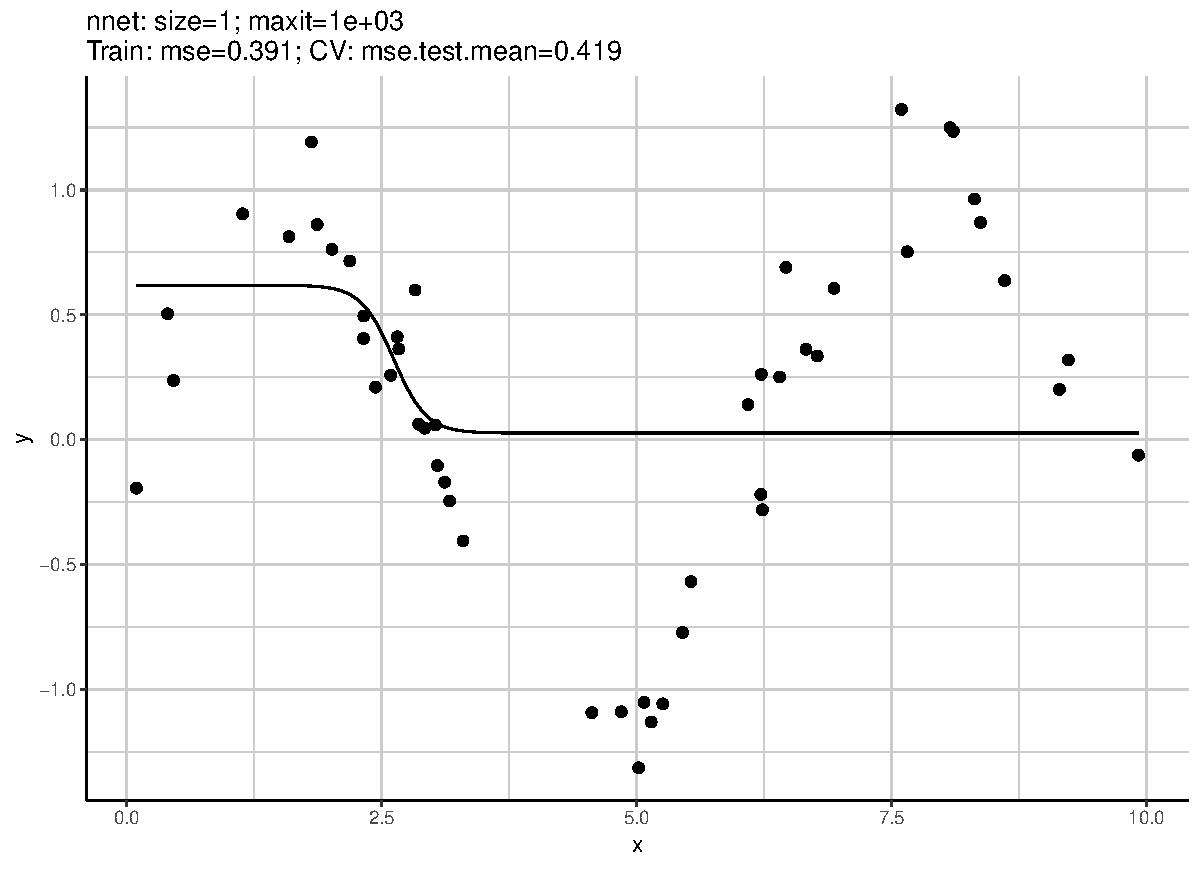
\includegraphics[width=0.95\textwidth]{figure/unnamed-chunk-5-1} 

}




{\centering 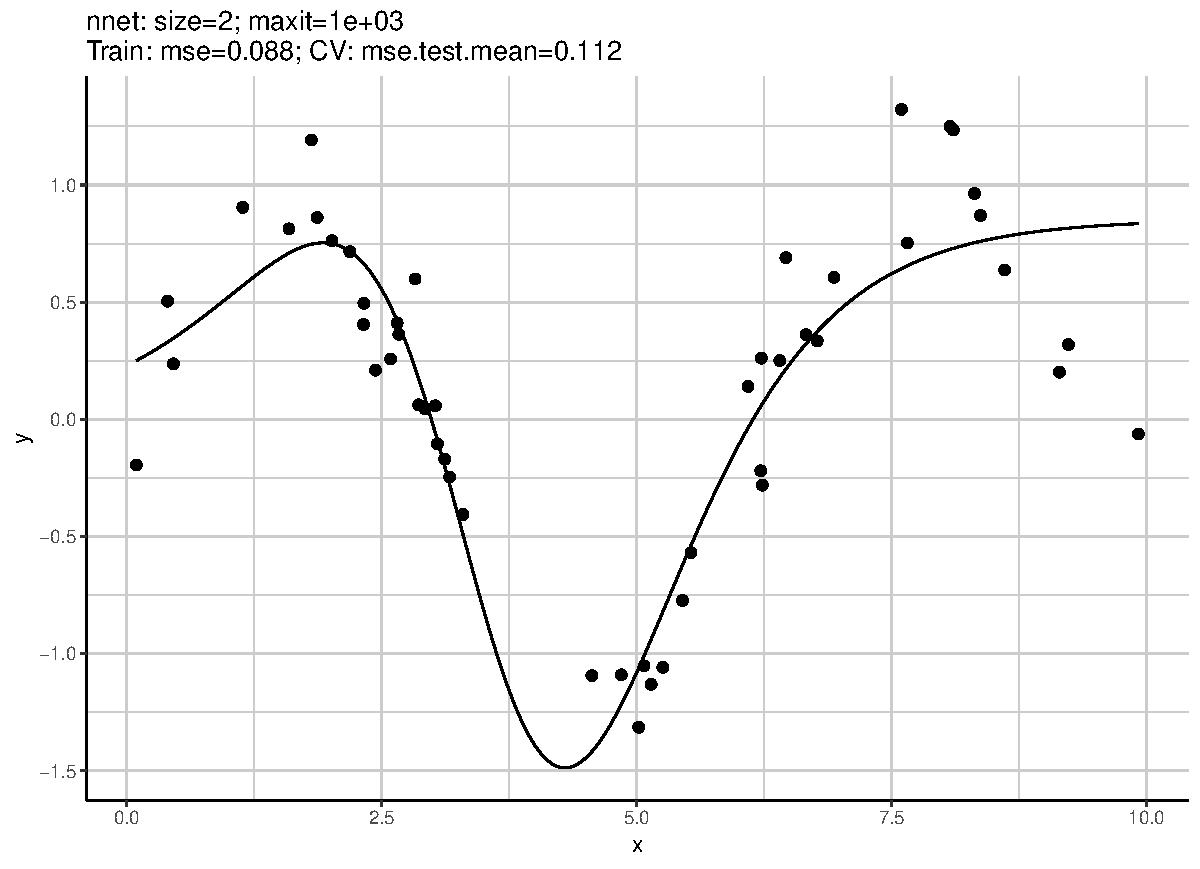
\includegraphics[width=0.95\textwidth]{figure/unnamed-chunk-5-2} 

}




{\centering 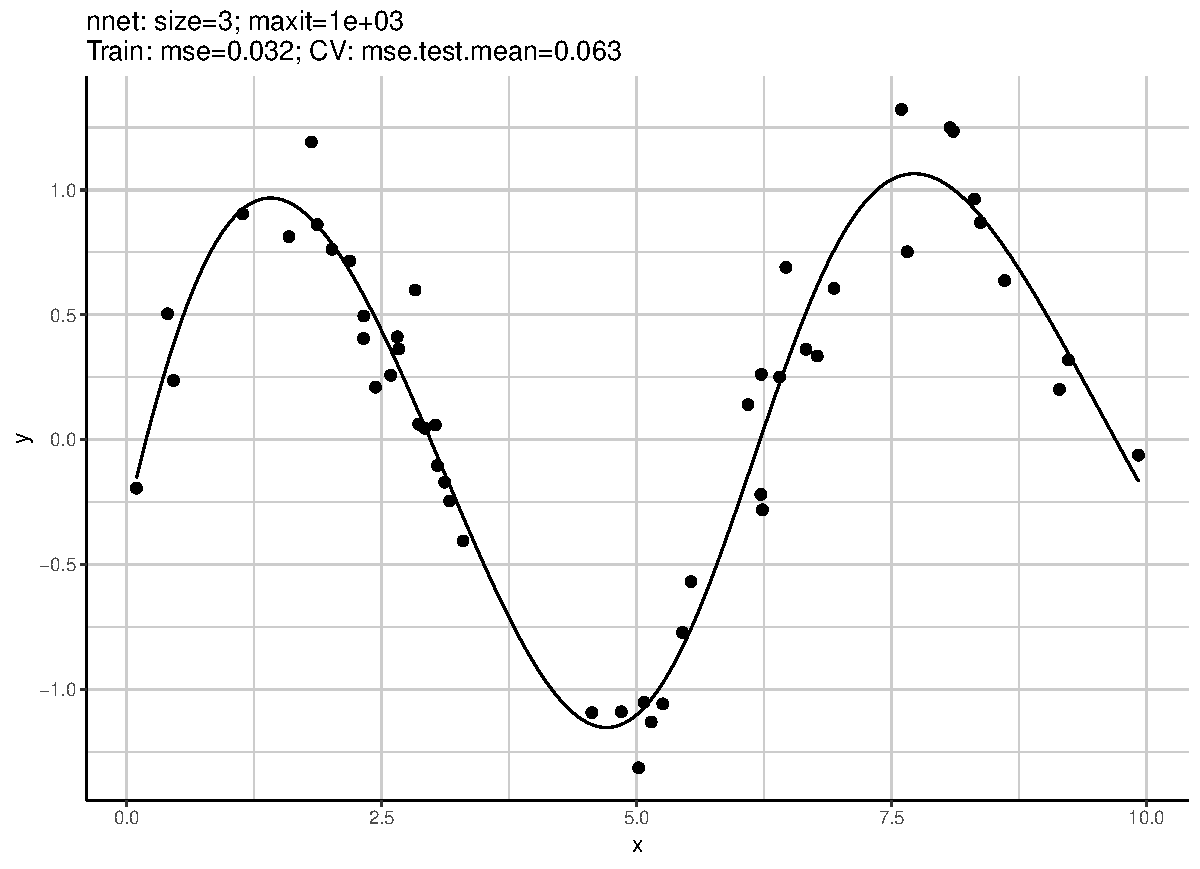
\includegraphics[width=0.95\textwidth]{figure/unnamed-chunk-5-3} 

}




{\centering 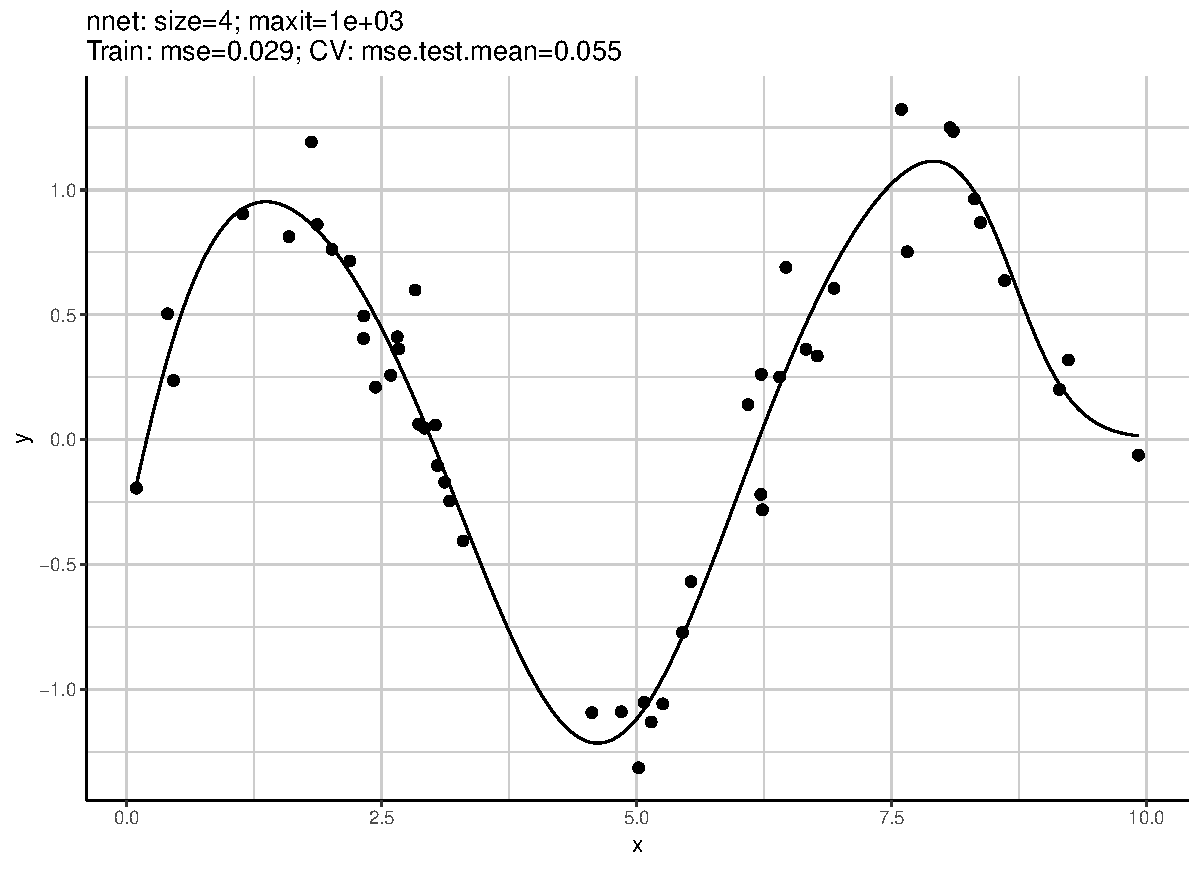
\includegraphics[width=0.95\textwidth]{figure/unnamed-chunk-5-4} 

}




{\centering 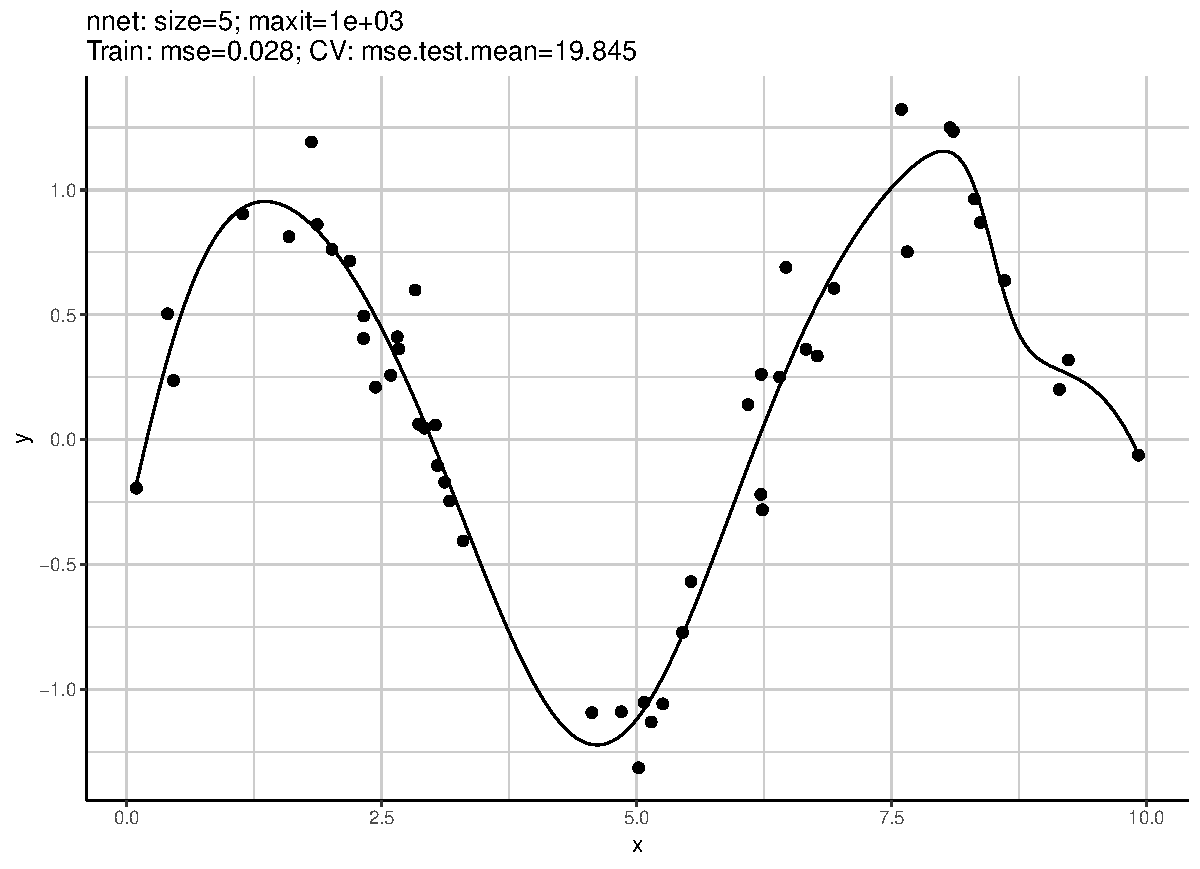
\includegraphics[width=0.95\textwidth]{figure/unnamed-chunk-5-5} 

}




{\centering 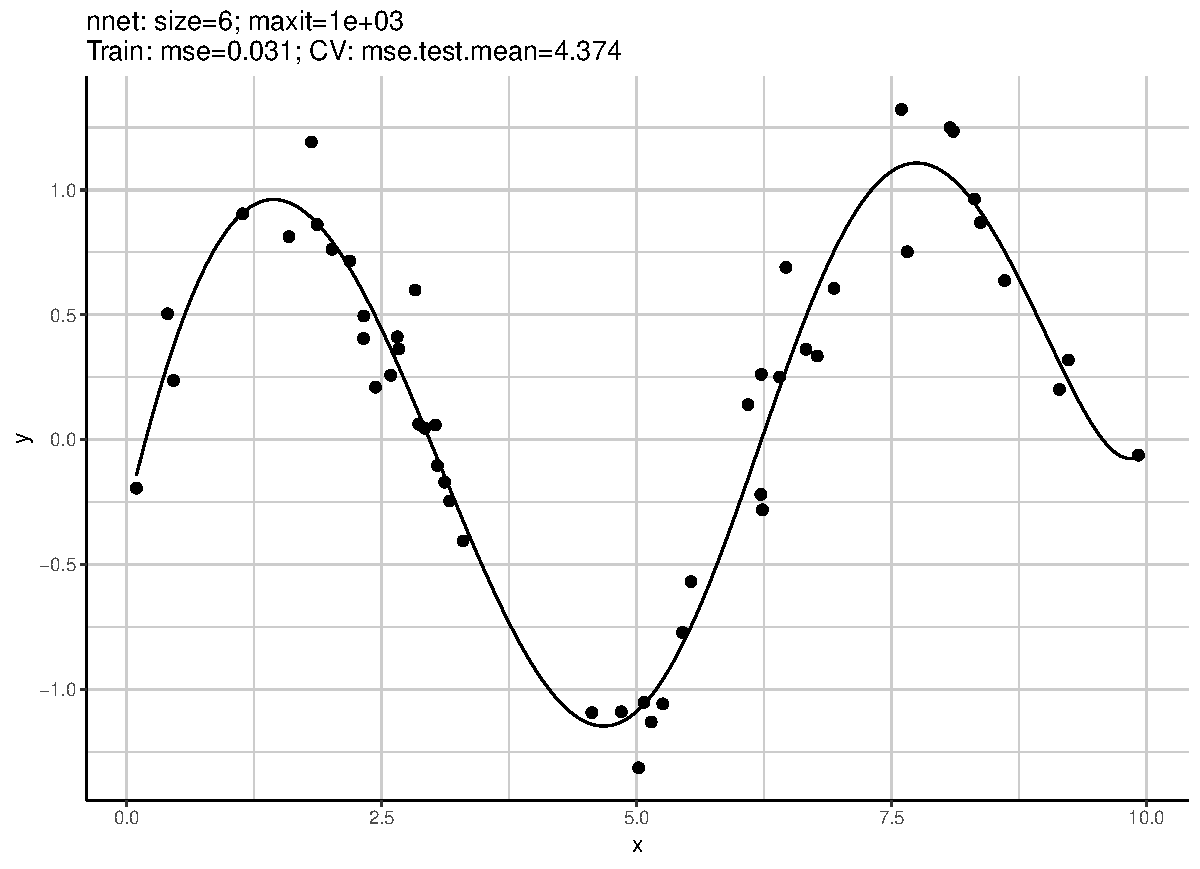
\includegraphics[width=0.95\textwidth]{figure/unnamed-chunk-5-6} 

}




{\centering 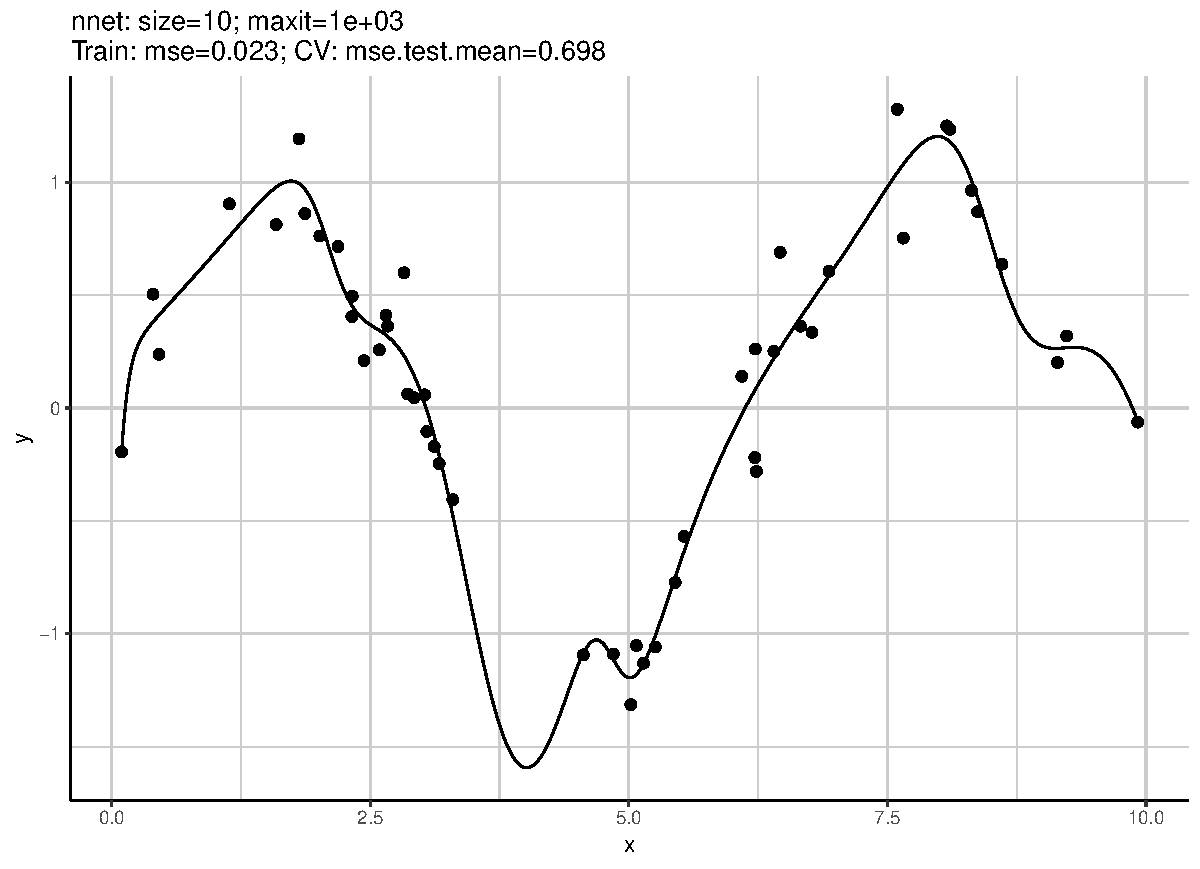
\includegraphics[width=0.95\textwidth]{figure/unnamed-chunk-5-7} 

}



\end{knitrout}
\end{vbframe}
%%%%%%%%%%%%%%%%%%%%%%%%%%%%%%%%%%%%%%%%%%%%%%%%%%%%%%%%%%%%%%%%%%
%%%%%%%%%%%%%%%%%%%%%%%%%%%%%%%%%%%%%%%%%%%%%%%%%%%%%%%%%%%%%%%%%%
\begin{frame}{Classification: 500 training iterations}

\only<1>{
\begin{knitrout}\scriptsize
\definecolor{shadecolor}{rgb}{0.969, 0.969, 0.969}\color{fgcolor}

{\centering 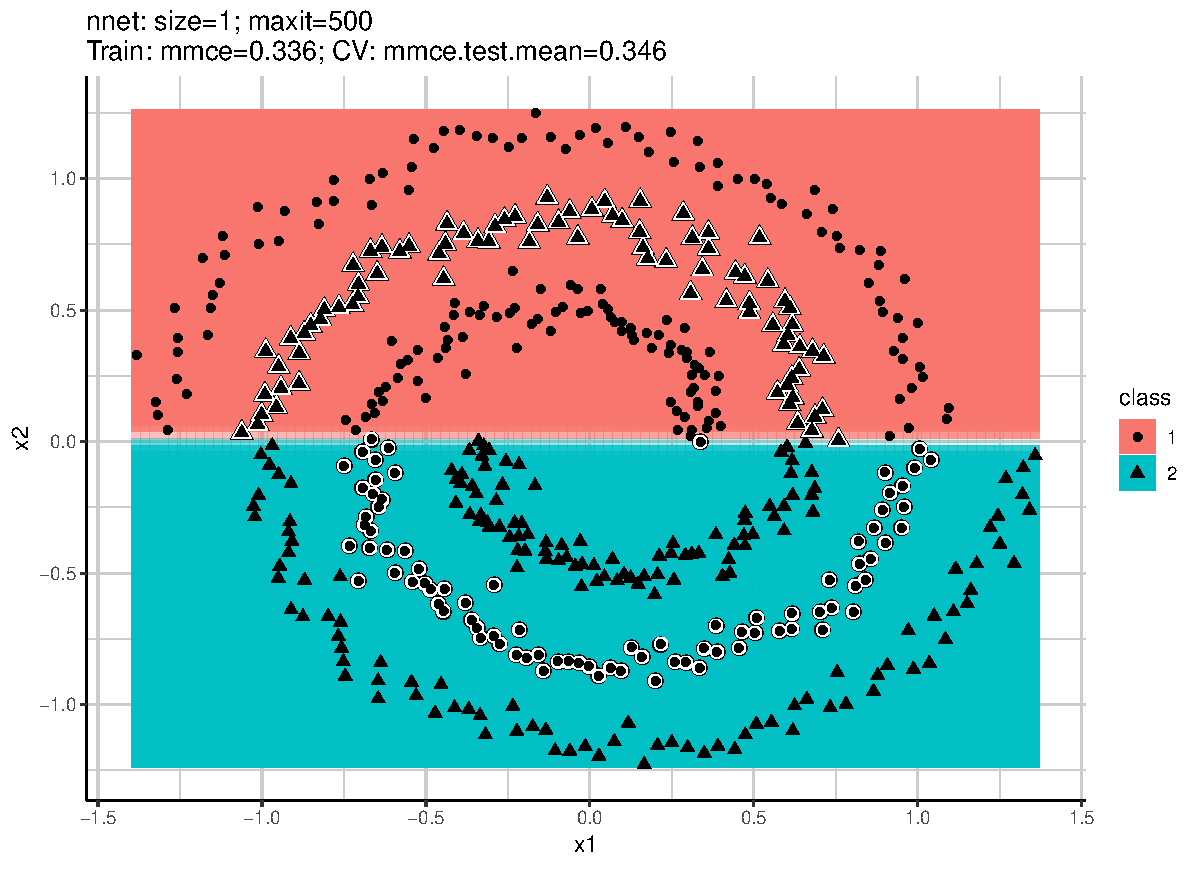
\includegraphics[width=0.95\textwidth]{figure/unnamed-chunk-6-1} 

}



\end{knitrout}
}

\only<2>{
\begin{knitrout}\scriptsize
\definecolor{shadecolor}{rgb}{0.969, 0.969, 0.969}\color{fgcolor}

{\centering 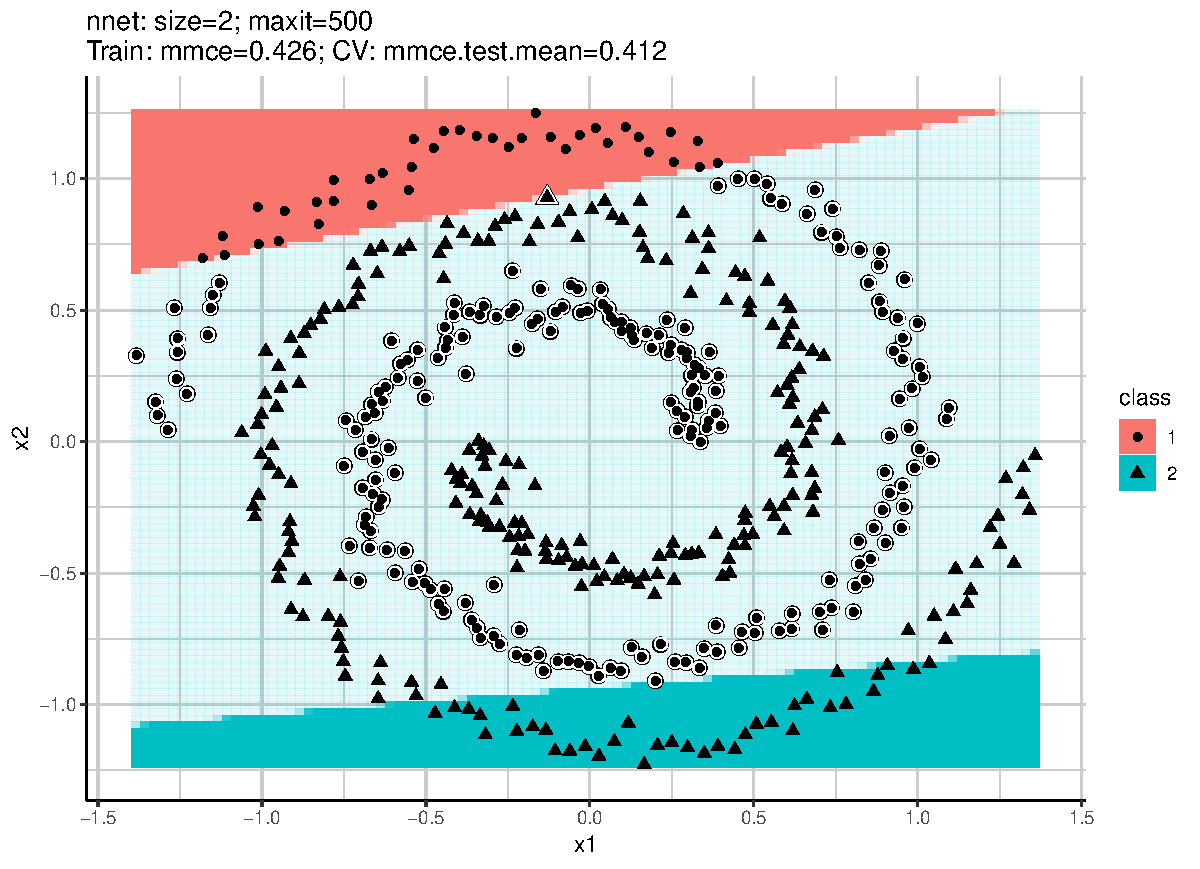
\includegraphics[width=0.95\textwidth]{figure/unnamed-chunk-7-1} 

}



\end{knitrout}
}

\only<3>{
\begin{knitrout}\scriptsize
\definecolor{shadecolor}{rgb}{0.969, 0.969, 0.969}\color{fgcolor}

{\centering 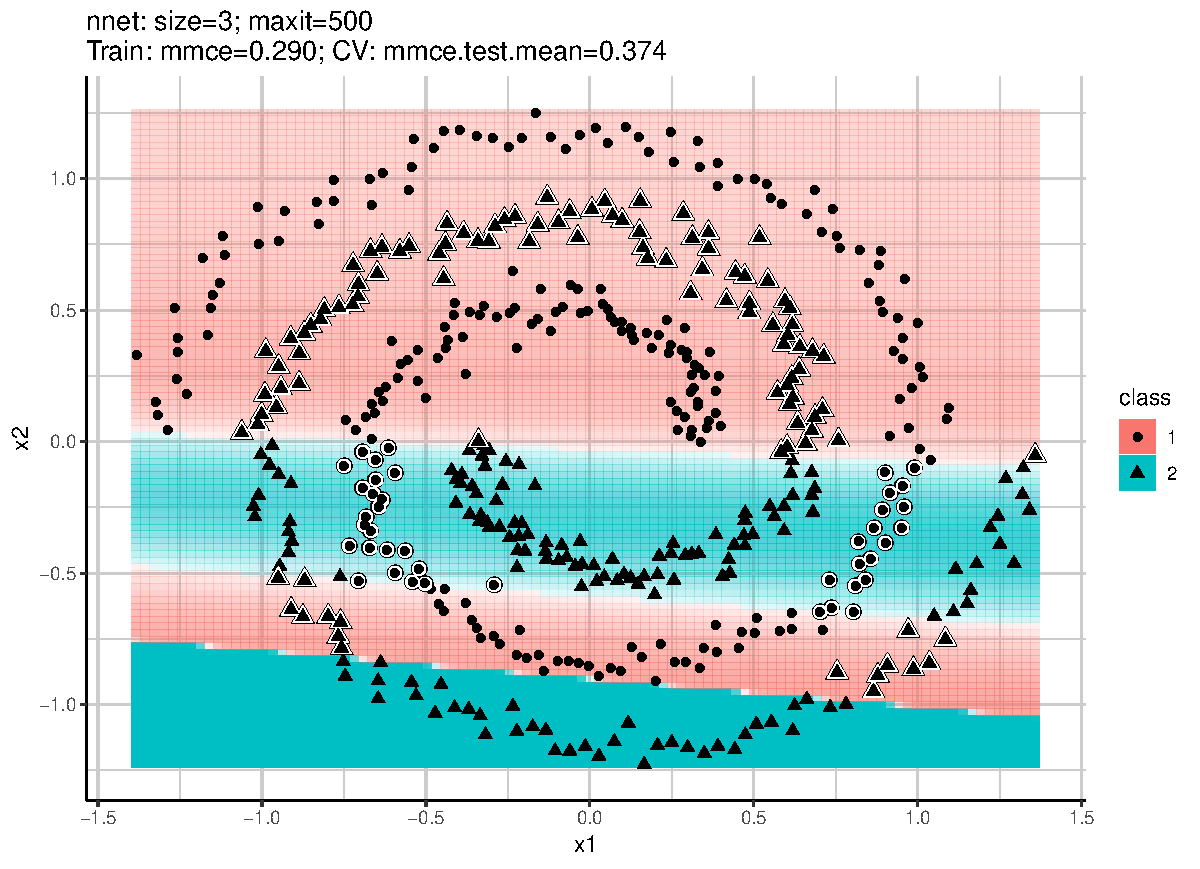
\includegraphics[width=0.95\textwidth]{figure/unnamed-chunk-8-1} 

}



\end{knitrout}
}

\only<4>{
\begin{knitrout}\scriptsize
\definecolor{shadecolor}{rgb}{0.969, 0.969, 0.969}\color{fgcolor}

{\centering 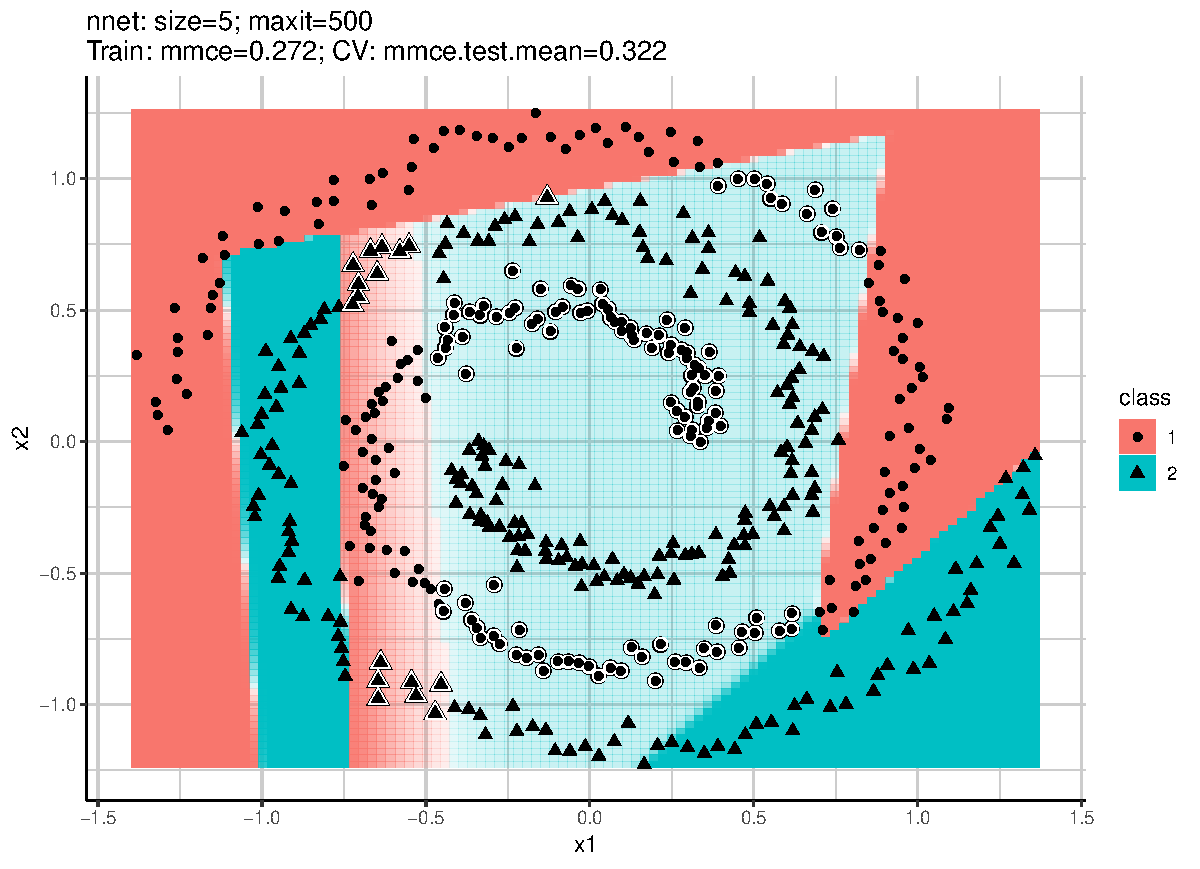
\includegraphics[width=0.95\textwidth]{figure/unnamed-chunk-9-1} 

}



\end{knitrout}
}

\only<5>{
\begin{knitrout}\scriptsize
\definecolor{shadecolor}{rgb}{0.969, 0.969, 0.969}\color{fgcolor}

{\centering 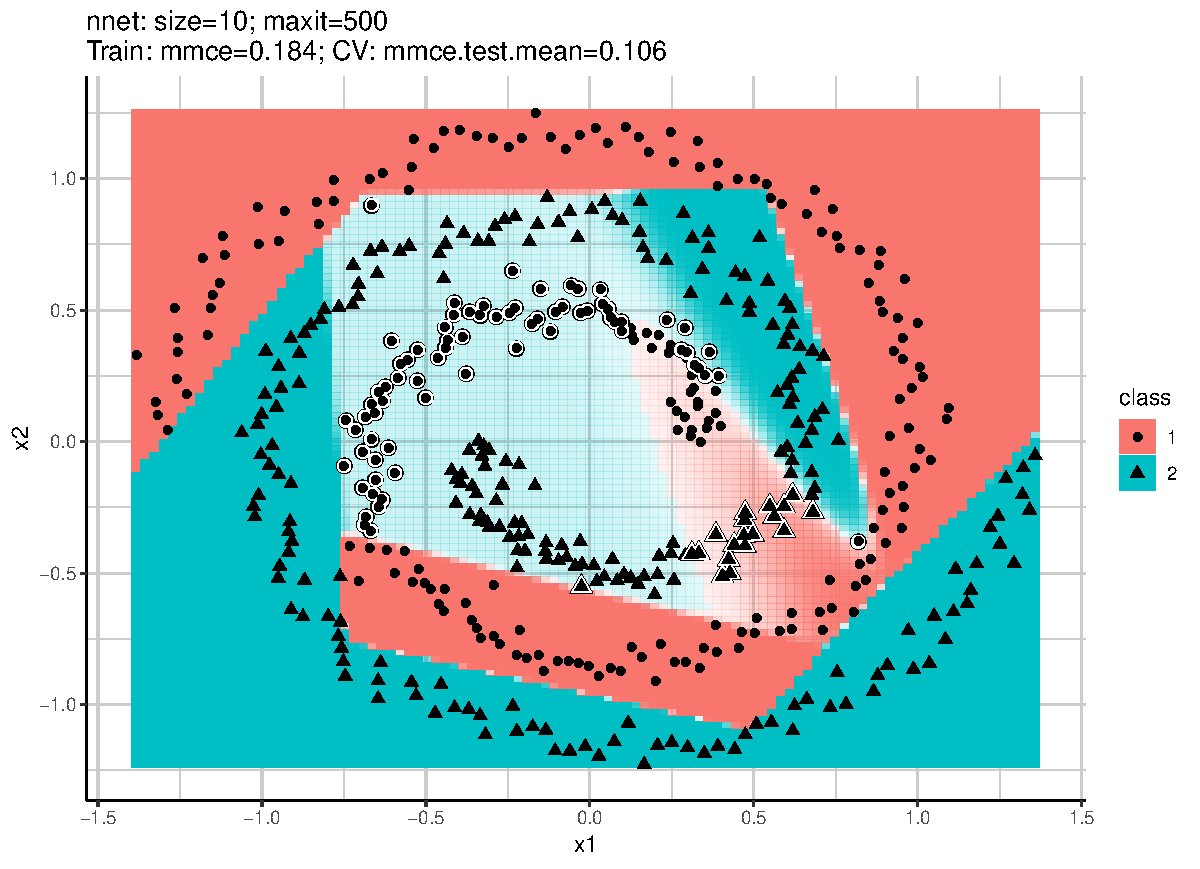
\includegraphics[width=0.95\textwidth]{figure/unnamed-chunk-10-1} 

}



\end{knitrout}
}

\only<6>{
\begin{knitrout}\scriptsize
\definecolor{shadecolor}{rgb}{0.969, 0.969, 0.969}\color{fgcolor}

{\centering 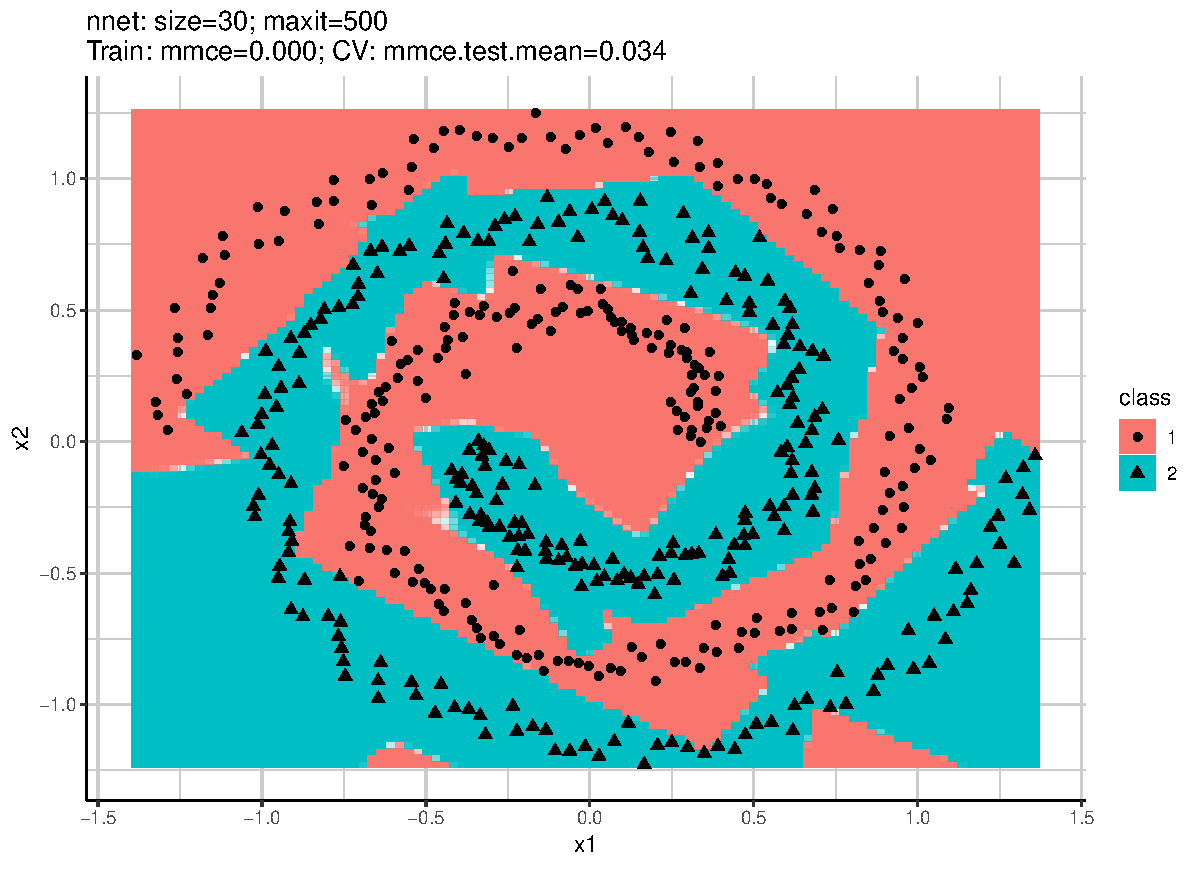
\includegraphics[width=0.95\textwidth]{figure/unnamed-chunk-11-1} 

}



\end{knitrout}
}

\only<7>{
\begin{knitrout}\scriptsize
\definecolor{shadecolor}{rgb}{0.969, 0.969, 0.969}\color{fgcolor}

{\centering 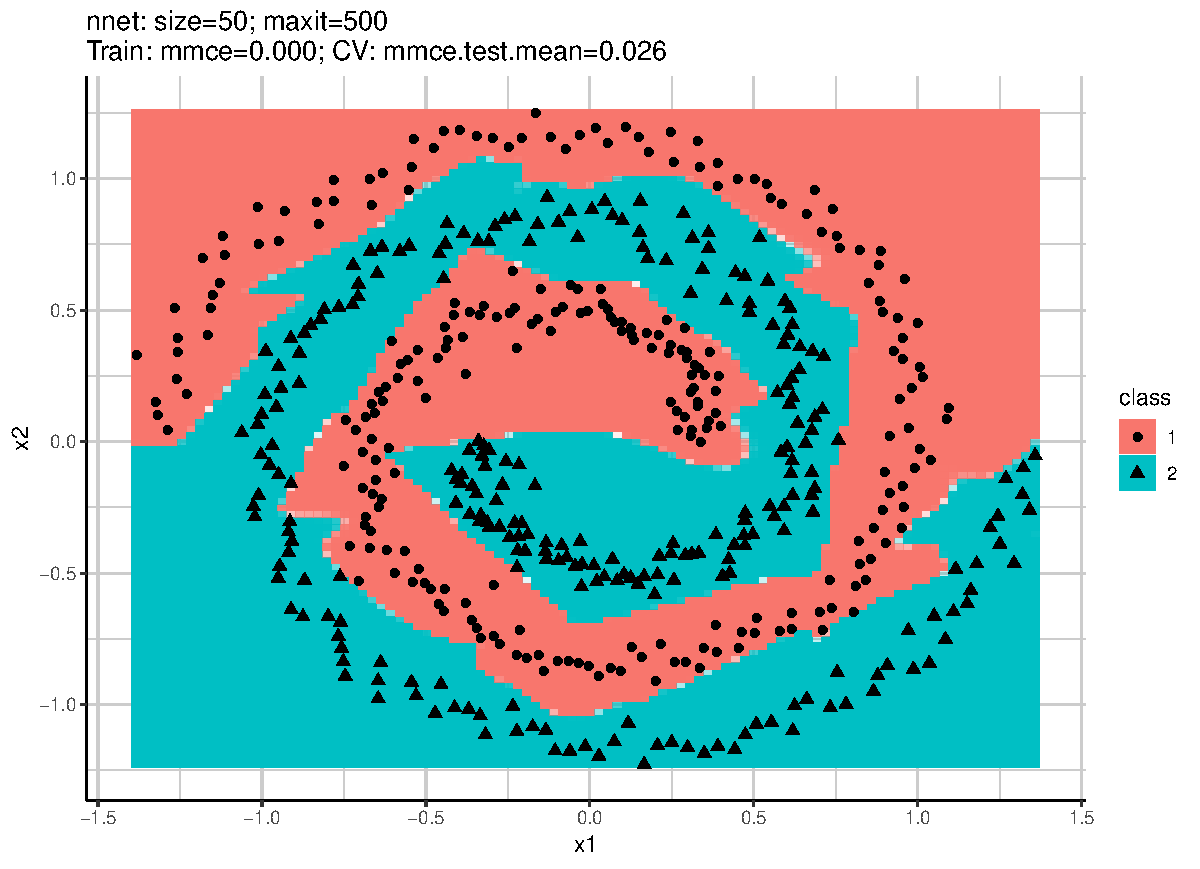
\includegraphics[width=0.95\textwidth]{figure/unnamed-chunk-12-1} 

}



\end{knitrout}
}

\end{frame}
%%%%%%%%%%%%%%%%%%%%%

\endlecture
\end{document}